\documentclass[12pt,a4paper,oneside]{article}
\usepackage[total={170mm,250mm}]{geometry}
% Toward automatic robot programming: learning human skill from visual data
\usepackage{graphicx}
\usepackage{multicol}
\usepackage{multirow}
\usepackage[]{natbib}
\usepackage{subfiles}
\usepackage{booktabs}
\usepackage{amsmath}
\usepackage{amssymb}
\usepackage{subcaption}
\usepackage{adjustbox}
\usepackage{array}
\usepackage{caption}

\usepackage{pdflscape}
\usepackage{lineno}
%\linenumbers
\usepackage{hyperref}


\usepackage{authblk}

\usepackage[table]{xcolor}

\usepackage[shortlabels]{enumitem}
\setlist[enumerate]{nosep}

\usepackage{tikz}
\usepackage{pgfplots}
\usetikzlibrary{calc}
\usetikzlibrary{patterns}
\usetikzlibrary{decorations.text}
\usetikzlibrary{shapes,snakes}


\usepackage{subfiles} 
\usepackage{natbib}
\newcommand{\SensorSubSec}[1]{ \vspace{0.5em} \noindent \textit{#1}}

\def\checkmark{\tikz\fill[scale=0.4](0,.35) -- (.25,0) -- (1,.7) -- (.25,.15) -- cycle;} 

\date{\vspace{10ex}}

%
\graphicspath{{./Diagrams/}{./Images/}}
%
\title{From art to part: learning from the traditional smith in developing flexible sheet metal forming processes}


\begin{document}

\author[1]{D. Bowen}
\author[2]{I. M. Russo}
\author[2]{C. Cleaver}
\author[2]{J. Allwood}
\author[1]{E. Loukaides}
\affil[1]{Department of Mechanical Engineering, University of Bath}
\affil[2]{Department of Engineering, University of Cambridge}

\maketitle


\begin{abstract}
The traditional metal smith has the remarkable capability to skilfully form a variety of part shapes from initially flat sheets, using only a few universal tools. Such versatility is increasingly appealing to manufacturers who now seek to diversify part catalogues and reduce tooling costs. Despite this utility, the laborious, manual nature of these traditional processes preclude them from meeting modern day high volume demand. However, these inefficiencies can be overcome through mechanisation with some traditional techniques being used as starting points in the development of new flexible processes. Here, we look at some of the techniques used by traditional craftsmen to form metal sheets and review different mechanised adaptations of these processes, focusing on the sensors and control systems used to operate the processes. We find these mechanised processes not yet as capable as their manual counterparts, suggesting there is still a lot we can learn from the craftsman. As such, we look both within and beyond the domain of metal forming at technologies and methods that can be used to capture the skilled actions of craftsmen and how this data can be used to enhance the design and operation of mechanised variants.

\end{abstract}
%\tableofcontents

\newpage

\section{Introduction}
%Recent manufacturing trends indicate a return to demand for a more diversified and personalised catalogue of parts, akin to that of the pre-industrial craft production era \citep{Koren2010TheRevolution}. This shift has been observed in the sheet metal forming sector \citep{Lee2012CaseTechnique} and has subsequently motivated development of new, more flexible manufacturing processes throughout both industry and academia \citep{Allwood2006AJapan,Yang2018FlexibilityForming}. However, developing these new flexible processes can be a challenging and complex task. Acknowledging the versatility and resourcefulness of the traditional metal smith, we look back at the tools and techniques that enabled them to form a diverse range of parts and see how this might be of use to modern process designers.

Traditional metal smiths were one of many groups of craftsmen described as \textit{``Skilled workers, using general-purpose machines, making exactly what the customer paid for; one product at a time''} \citep{Koren2010TheRevolution}. Working in isolation in small shops, these skilled workers were responsible for the design, manufacture and assembly of the relatively simple goods compared with modern products \citep{Groover2015AutomationEdition}.  Using only a small number of tools and techniques, these traditional craftsmen were capable of forming a diverse range of parts from initially flat sheets. Crucially, these parts were the product of human effort and skill, with ability to create desired forms consisting for the most part a combination of manual dexterity and following a large number of intuitive, empirical rules derived from an evolved understanding through experience \citep{Hall1961EngineeringRevolution}. Traditional techniques developed by the smith have been used in modern day, high value, low volume production of sheet metal parts \citep{Amos2015Bloodhoundfeathers}.

\begin{figure}[h]
	\centering
	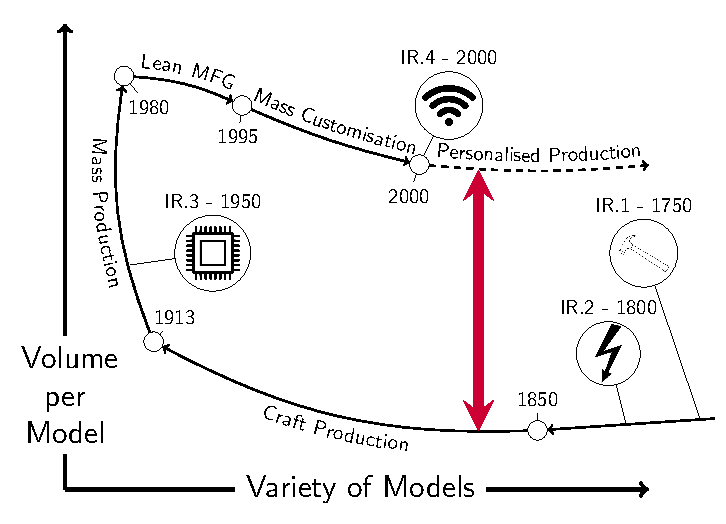
\includegraphics[scale=0.75]{MfgPatterns_V3.pdf}
	\caption{Demand for volumes and varieties of parts, subsequent manufacturing paradigms and defining technologies of industrial revolutions (IR), showing the current demand for part varieties were obtainable by the craftsman, but are now required at far greater volumes.}
	\label{fig:VarietyVolume}
\end{figure}

Despite its versatility, the time-consuming and labour intensive nature of craft production renders it unsuitable for modern day industrial scale use, which requires highly efficient processes to meet high-volume demand. This is illustrated in Figure \ref{fig:VarietyVolume} which chronologically maps the changes in market demand over the past century  along with industrial revolutions (IR), and corresponding manufacturing paradigms whose technology invoked and/or enabled these shifts in demand. By combining qualitative perspectives from the literature \citep{Koren2010TheRevolution,Popkova2019FundamentalRevolutions,Mourtzis2012DecentralizedOutlook,Mourtzis2014TheCustomisation}, it shows that the market is entering an era of personalised production, demanding high-volume production of an ever broader variety of parts. 

For the metal forming sector, this demand for high volume and highly personalised production has motivated development of flexible processes, characterised by the ability to produce an extended range of part geometries without the need for part specific tooling. These flexible metal forming systems provide a more cost effective and sustainable method of production to meet these new demands when compared with using typical mass-production metal forming processes which require bespoke tooling, producing substantial waste in the form of discarded materials and workpiece offal, alongside incurred storage and development costs \citep{Cooper2017TheProcesses,Horton2019ImplementingComponents}. The design of hardware and suitable control software for flexible metal forming systems is a topical but challenging task. Due to the stochastic and non-linear nature of the material properties, conventional systems typically require complex control systems, advanced planning and closed-loop control to achieve high quality single part forms  \citep{Allwood2016Closed-loopForming, Tekkaya2015MetalProperties, Polyblank2014Closed-loopProspectus}. The addition of degrees of freedom in flexible systems exacerbates these problems. 

One solution to this issue is to automate some of the techniques used by traditional metal smith, using modern technologies to bridge the chasm of productivity (Figure \ref{fig:VarietyVolume}) whilst retaining the aforementioned versatility. Mechanising manual processes is often straightforward and can often be done using off-the-shelf industrial robot arms which can match and surpass human physical and dexterous capabilities - strength, range, positioning accuracy; for a useful definition of automation of physical tasks see Frohm \citep{Frohm2008LevelsManufacturing}). However there is no straightforward procedure to replicate the craftsman's logic in controlling these process to produce desired parts. In  Frohm's definition, this is analogous of the automation of cognitive tasks. This suggests any gap in utility between automated processes and their manual counterpart likely lies in the control and operation of these processes.

The skilled intuition of the craftsman that enables such versatility is built up over many years and is hard to digitally replicate. However computers are becoming increasingly efficient at acquiring human skills, especially when large amounts of training data is available \citep{Ford2016TheUnemployment}. This new data driven approach to process control is aligned with the next industrial revolution - I4.0 \citep{Zhong2017IntelligentReview}. % Many more citations could be included here to emphasise/expand the point.
As designers often do not revisit the craftsman throughout the development of these new processes, this implies large amounts of knowledge are discarded by not looking at how the craftsman operates these processes. This represents a missed opportunity to develop new approaches to these challenges using technologies from within and outside metal forming to capture and transfer data from skilled humans to intelligent systems which enable autonomous forming machines.

This part paper aims to respectively motivate, review and advance the mechanisation and automation of traditional sheet metal forming processes. Section \ref{sec:Manual} looks more closely at the traditional metal smith; it specifically focuses on four tools and some common techniques used to form sheet metal, demonstrating their versatility and providing motivation for the mechanisation of these processes. Section \ref{sec:Mechanised} reviews the state of the art for flexible processes that are based on these manual tools and techniques, highlighting both the control systems and mechanical configurations used. Finally, Section \ref{sec:Learning} looks both within and beyond the metal forming domain at ways in which designers can further learn from skilled craftsmen in both the design and operation of these mechanised processes.


\newpage
\section{Manual Sheet Forming}\label{sec:Manual}
\subsection{Background}
Manual sheet forming, also known as ``panel beating'' or ``coach building'' encompasses a number of manual processes used by skilled workers to form curved parts from initially flat aluminium and steel sheets. The traditional smith skilfully forms the material using a range of tools and techniques in a specific order of operations to incrementally bend and/or stretch/shrink across the face of the sheet, the latter resulting in curvature as a consequence of Gauss's Theorema Egregium \citep{Pressley2001ElementaryGeometry}.  At the same time, care is taken to maintain control over the thickness of the part, the emergence of wrinkles and the mechanical properties of the material. These methods of production enable inherently versatile manufacturing where part forms can be changed easily.

Typical parts manufactured using these processes include non-load-bearing panels for the automotive, aerospace and architectural industries, the geometries of which can be complex and include double curvature. Pre-dating the era of increased automation and high volume production, panels were often formed by these skilled craftsmen in large factories - Figure \ref{fig:OldFactory}. Becoming fully competent in the art of panel forming takes around 10 years of training \citep{Goodwin2020BehindBeaters}. The acquired skill set also equips them with the ability to repair damaged panels, with substantial implications for the servicing of a large range of products. . However, the manual and laborious nature of this process results in a timely and inefficient means of production.

These flexible techniques have since been replaced with faster, more rigid processes to cope with demand. Alongside reduced flexibility, one of the unintended consequences of this change was the loss of the underlying expertise in the manipulation of sheet metal geometry - the art of crafting.  Despite this decline in the number of skilled, professional smiths, the art of manual sheet forming is kept alive through a small community of enthusiasts and small number of job shops. 

The worker typically controls both the movement of the tooling and the workpiece in these processes. Unlike industrialised metal forming, there is no rigorous classification of processes that are used by the panel beater. Given the colloquial language used to describe craft techniques and the ad hoc nature of some processes, creating a taxonomy would be challenging. Instead, we review common techniques used in forming different sheet metal geometries, grouped by the tooling used to carry out the process. We describe the fundamental techniques that are used to form material, the underlying mechanics of the process and the typical geometries that are produced. 


\begin{figure}[h]
	\centering
	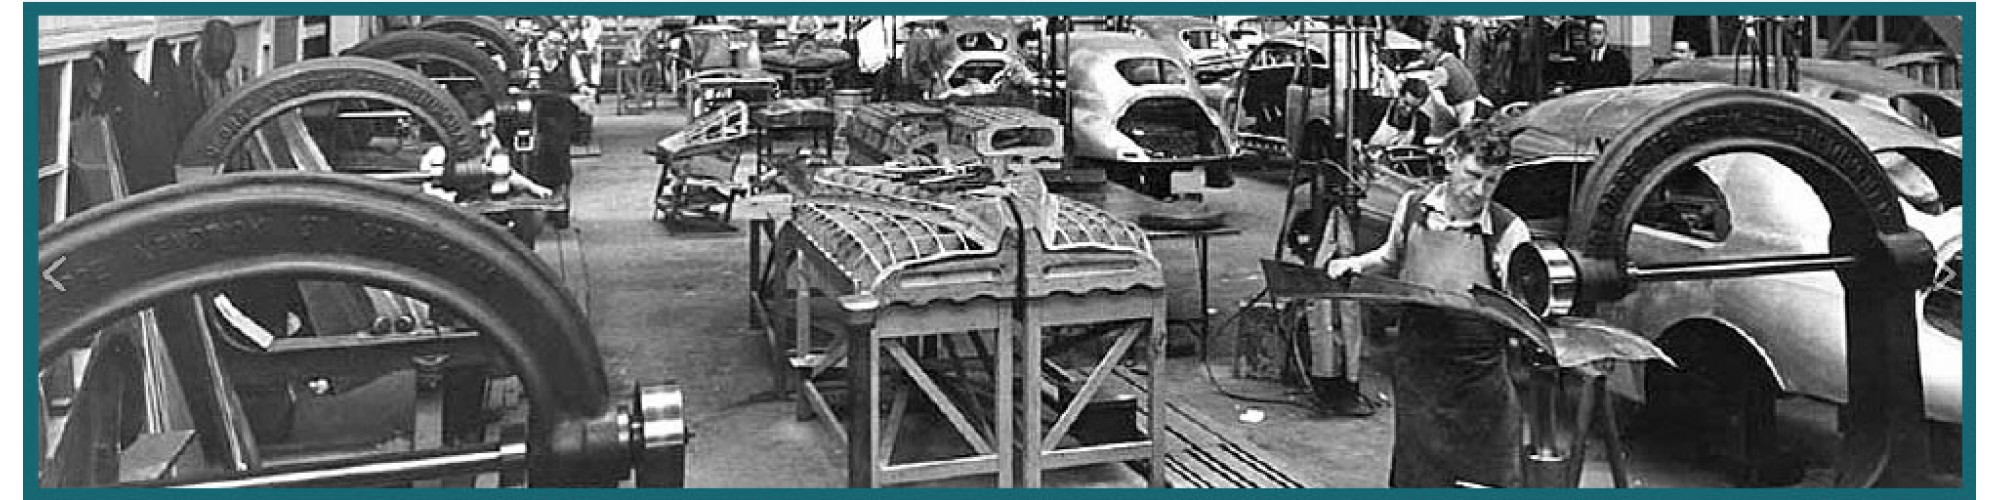
\includegraphics[width=0.9\linewidth]{OldFactory.png}
	\caption{Panel Beating factory, circa 1920, accessed from \citep{clementandboggis2018}}
	\label{fig:OldFactory}
\end{figure}


\subsection{Tools and Processes} \label{sec:ToolsandProc}
\subsubsection*{Hammers}

Hammering is perhaps the most crude technique used by the smith in terms of tooling, but is by no means the least complex. In this category of processes, the worker strikes the sheet, squeezing material between the hammer head and a supporting anvil. The through-thickness compression causes thinning at the impact zone and spreads material outwards \citep{Music2012TheTools}. The desired profile is formed by incrementally working across the face of the sheet. There is no definitive list of hammer sizes/shapes and often hammers are personalized to both the workman and the job \citep{Barr2013ProfessionalFabrication}. Similarly, different anvils are used for jobs, such as wooden dollies, cast anvils or sandbags. Hammers and dollies are generally selected based on the technique used to form material, with the three main techniques used by panel beaters being hollowing, raising and planishing. 

\begin{figure}[h]
	\centering
    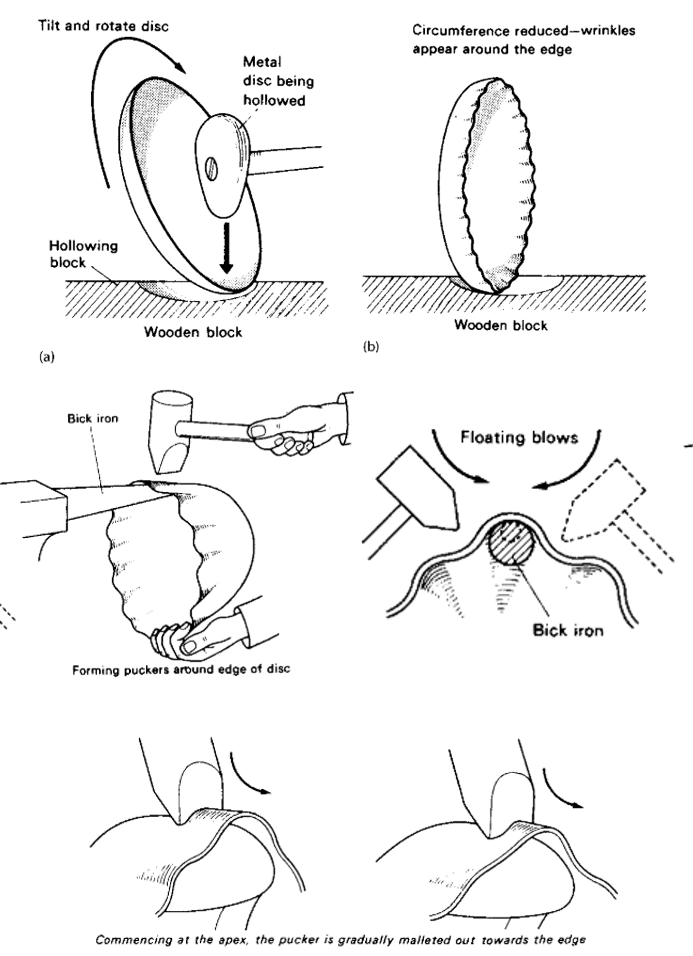
\includegraphics[width=0.4\linewidth]{HammeringTechTemp.png}
    \caption{Hammering Techniques}
    \label{fig:hammeringtechnique}
\end{figure}

Hollowing (sometimes called sinking) is perhaps the least complex hammering process and is used to form smaller compound curvatures or dishes - Fig \ref{fig:hammeringtechnique} a. The workpiece is held at an angle above a compliant sandbag or above a wooden anvil with a crevice. The material is then struck with a large head hammer, sinking the material into the crevice/bag. After each blow, the workpiece is rotated, and the process is repeated with each blow slightly overlapping the previous. Starting at the outer edge and working around the perimeter of the workpiece, blows slowly spiral toward the centre, resulting in a domed compound curvature shape. %EGL: CITATION? ALSO FOR FIGURE % DB: We are going to produce our own figures

Raising is a more complex hammering process that allows larger curvatures to be formed \citep{Livesey2019TheBodies}. To start, the workpiece is given a slight curvature by hollowing, and then placed onto the centre of a hard, pin shaped anvil. Using a smaller, heavier head hammer, material is struck just beyond the edge of the anvil, forcing it down and around the anvil and effectively shrinking or reducing the circumference of the workpiece. The workpiece is rotated and the process repeats, spiralling from the centre, to the outer edge. Wrinkles that arise from reducing the circumference are worked out by skilfully thickening the material by striking the base of the wrinkle, bringing together each sides of the wrinkle.  Raising can also be carried out by tucking the edges of the workpiece. This reduces the circumference by folding material at the edge over itself into a wrinkle using a two prong fork, then working the wrinkles out. % Needs better explaining - perhaps a diagram 

Smaller, flat-head hammers are used to planish imperfections from the surface of a worked sheet. By carefully striking high spots on the sheet, the material thins and spreads outwards, leaving an improved surface finish. A hard anvil is normally used during this process. There are several variations of planishing hammers called ``spoons'' and ``slappers'' which are suited to the task of planishing \citep{Barr2013ProfessionalFabrication}. The process can also be carried out using hand held dollies, allowing for repair work to be carried out, without having to remove panels or a ``bulls-eye pick'' can also be used for repair work, which mounts a hammer and anvil on a hinged C shaped jaw-frame which can be actuated at the base of the frame allowing the worker to access and planish difficult to access areas.


\subsubsection*{Kraftformer} \label{sec:Kraftformer}

The kraftformer machine is the commercial name for the more widely known `shrink/stretch machine' made by Eckold \citep{Unknown2020ECKOLDBrochure}. A C-shaped frame houses a reciprocating press that is actuated either manually by a food pedal or is mechanised where the depth of stroke and the number of strokes per minute can be adjusted. There are several types of tools of various sizes that can be fitted to the end of the press, each deforming the workpiece differently. When forming sheets, the stretching and shrinking tools are primarily used.

When \textit{driving} (the name given to the technique used when operating a Kraftformer), the craftsman stands beside the machine, with both hands holding the sheet and resting it between the jaws of the press. A schematic of the deformation process is shown in Figure \ref{fig:KraftformingProcess}. With each stroke, both the upper and lower tools are moved toward the sheet until the sheet is clamped. The remaining vertical motion of the stroke is translated into horizontal movement with the tools moving outward or inward, stretching or shrinking the sheet respectively.  As the press reciprocates, the workpiece is manoeuvred to incrementally form the face of the sheet along the desired path. This repeated stretching or shrinking action causes curvature to be developed and a global shape is formed. The maximum pressure that can be exerted on the sheet varies with different models of kraftformer and is proportional to the size of the machine. [We could cite http://www.klassictoolcrib.com/2018KTCMini.pdf ?]


\begin{figure}[h]
    \centering
    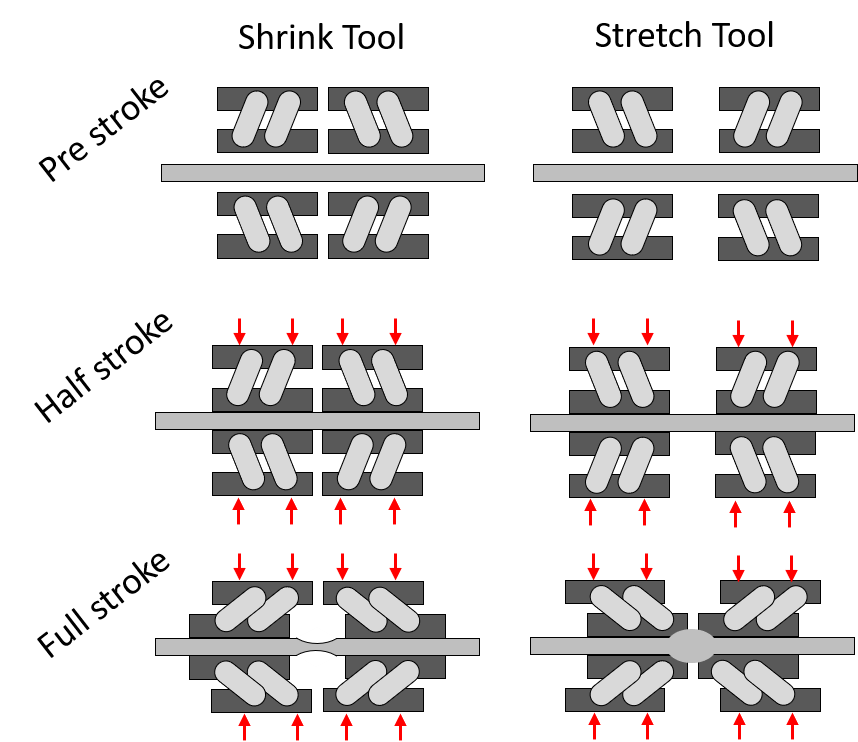
\includegraphics[width=0.45\linewidth]{KraftformingTechTemp.png}
    \label{fig:Kraftformer}
    \caption{Kraftformer Tool}
\end{figure}






\subsubsection*{English Wheel}

The English wheel, sometimes called a wheeling machine, is primarily used to form or planish sheets with compound curvatures. A typical wheel is shown in Figure \ref{fig:wheel_frame} and consists of a C-shaped frame, similar to a Kraftformer, with two anvil rollers. The upper anvil roller has a flat profile, whereas the lower is often crowned to accommodate for curvature in the sheet in the transverse to roll direction. The lower tool can be quickly changed to another tool with less/greater crown and the gap between the rollers finely adjusted using a leadscrew to change the height of the lower tool.

\textit{Wheeling} (the process of using an English wheel) is renowned as a complex task capable of fabricating intricate, smooth curves, whilst leaving an aesthetically pleasing finish and good surface quality \citep{Longyard2014LearningWheel}. Similar to \textit{driving}, the worker stands beside the machine with both hands on the sheet and places the sheet between the rollers. By raising the lower anvil roller, the sheet is pinched between the two rollers. The worker then manoeuvres the sheet back and forth between the two anvil rollers, tracking across the face of the sheet in a `zig-zag' pattern. Back and forth strokes should slightly overlap and the pressure on the sheet should not be excessive to ensure a quality finish. 

The deformation at the tools is a combination of stretching and bending with the anvils incrementally, continually thinning the material, stretching material outward away from the tools \citep{Music2012TheTools}. The trajectory and density of back and forth strokes, as well as various machine parameter settings (roll gap, lower anvil shape) all impact the change the way the sheet forms [CITE ICTP paper]. When \textit{wheeling}, an outer boundary on the sheet face is left unwheeled, constraining the stretched material and causing the inner region to rise out of plane, resulting in compounded curvature. Being acting as a stretching tool, the English Wheel is often used to planish wrinkles from previous operations, such as hammering, or as an embossing tool.


\subsubsection*{Spinning}
Hand spinning is a process in which a craftsman forms axially symmetric parts from initially flat metal sheets using a lathe and a manually held tool. A mandrel shaped to the desired profile (also known as “chuck” or “former”) is mounted to the headstock of a spinning lathe and a blank workpiece is mounted in line and held in place with a follower, clamped by the tailstock. With both the workpiece and follower rotating, the craftsman applies pressure to the workpiece using a forming tool, traversing from the centre of the blank to its outer perimeter and back in rapid strokes. This causes the workpiece to progressively flow and eventually take the shape of the mandrel. 

When spinning, the craftsman stands beside the machine and has control over both the rotational velocity of the spindle and the trajectory of the forming tool. There is no standardised set of tooling used in spinning and craftsman often create their own tooling tailored for the job. However, tools are typically long metal sticks with a suitable geometry at one end and a wooden handle at the other. They are used to perform functions such as forming, cutting and polishing. A tee-rest with a moveable fulcrum pin allow the craftsman to apply high forces while maintaining control over the motion of the tool, and to move forwards axially as the workpiece takes shape. A wooden backstick is also commonly used during the forming stage to prevent wrinkling of the workpiece, which is especially likely when the blank is thin \citep{Jawale2019AnSpinning}. Lubrication is routinely used to reduce heating, make the forming easier and avoid scratching the workpiece. 

As explained at length in old manuals \citet{Holtzappfel1852TurningManipulation,Tuells1912MetalUsed}, many years of practice are required for spinning craftsmen to consistently achieve success for a variety of geometries and materials. The overall perimeter of the workpiece from the initial to the final shape must decrease, which makes it prone to circumferential buckling. This can be balanced by allowing the workpiece to elongate radially, but excessive elongation leads to tearing. Thus, the craft of spinning consists in progressively forming the blank while avoiding both wrinkling and excessive elongation. The shape of the workpiece, its resistance to deformation and the sounds it makes are all cues for the craftsman to understand how to successfully form it. 

\begin{figure}[b]
\begin{subfigure}[b]{.23\linewidth}
	\centering
    \includegraphics[width=0.8\textwidth]{example-image-b}
    \caption{Hammering}
    \label{fig:HammeringProcess}
\end{subfigure}
%
\begin{subfigure}[b]{.23\linewidth}
	\centering
    \includegraphics[width=0.8\textwidth]{example-image-b}
	\caption{English Wheel}
	\label{fig:WheelingProcess}
\end{subfigure}
%
\begin{subfigure}[b]{.23\linewidth}
	\centering
	\includegraphics[width=0.8\textwidth]{example-image-b}
    \caption{Kraftforming}
	\label{fig:KraftformingProcess}
\end{subfigure}
%
\begin{subfigure}[b]{.23\linewidth}
	\centering
    \includegraphics[width=0.8\textwidth]{example-image-b}
	\caption{Spinning}
	\label{fig:SpinningProcess}
\end{subfigure}
\caption{Manual Metalforming Techniques}
\label{fig:ManualTech}
\end{figure}



\subsection{The craftsman's tacit knowledge} \label{sec:tacitknowledge}

The geometry of parts produced by panel beaters are often made from a variety of constituent complex shapes. As each of the techniques described in section \ref{sec:ToolsandProc} will have a unique, constrained range of possible geometries that can be formed from the preformed panel - created in an earlier process, forming the overall shape often requires multiple incremental operations, utilising multiple techniques. For example, in the production of a motorcycle fuel tank (a commonly used example project in training manuals) a combination of hollowing, raising and wheeling can be used to form the shape as well as other auxiliary processes such as cutting, welding and finishing operations \citep{Barr2013ProfessionalFabrication}. Successful production requires both correct selection and operation of these different processes. 

When considering an automated solution for universal part production with craft inspired processes, using multiple tools/techniques will likely be necessary. This would currently be a complex and challenging task as autonomous variants of individual processes alone are still underdeveloped, with process capabilities not rigorously defined and with poor repeatability. Furthermore, automated methods for flexible process selection are in their infancy \citep{Hamouche2018ClassificationLearning}. However, the craftsman still has the capability to form a range of shapes using only a single technique. In line with reviewing the physical tools and techniques used by the craftsman, it is also valuable to consider the craftsman's cognitive process when crafting, so this too might be replicated in the design of an equivalent autonomous process machine.

Consider the craftsman using a hammer to hollow a dome from a flat sheet as described in \citep{Barr2013ProfessionalFabrication}. In this process, there are three main elements: the workpiece to be deformed, the tool(s) to carry out the deformation and the craftsman, who provides controlled actuation of both tool and workpiece. The worker is a source of both energy (in the form of manual actuation) and information (in the form of a decisive strategy), the combination of which gives controlled movement of both the tool and workpiece in a trajectory described as a manufacturing strategy. Through the tool, energy is exchanged into the workpiece causing deformation, with some being exchanged into the surrounding environment (as sound and heat etc.). In some crafts such as spinning or driving, the energy used to deform is sourced from the tool and is regulated and controlled by the worker. Energy is also used to manually manoeuvre the workpiece. Throughout crafting, the worker continuously receives feedback from everything they are interacting with: the tool, workpiece and environment. 

Employing this gathered information, a design activity pattern for craft sheet forming is mapped in Figure \ref{fig:DAP}. Similar analysis has been done for other manufacturing processes and systems. For example, using this approach \citep{Roth1981FoundationDesign} constructed a model of manual wood cutting and \cite{Zhou2018TowardManufacturing} applied the same concept to a Human-Physical system. 

\begin{figure}[h]
  \centering
  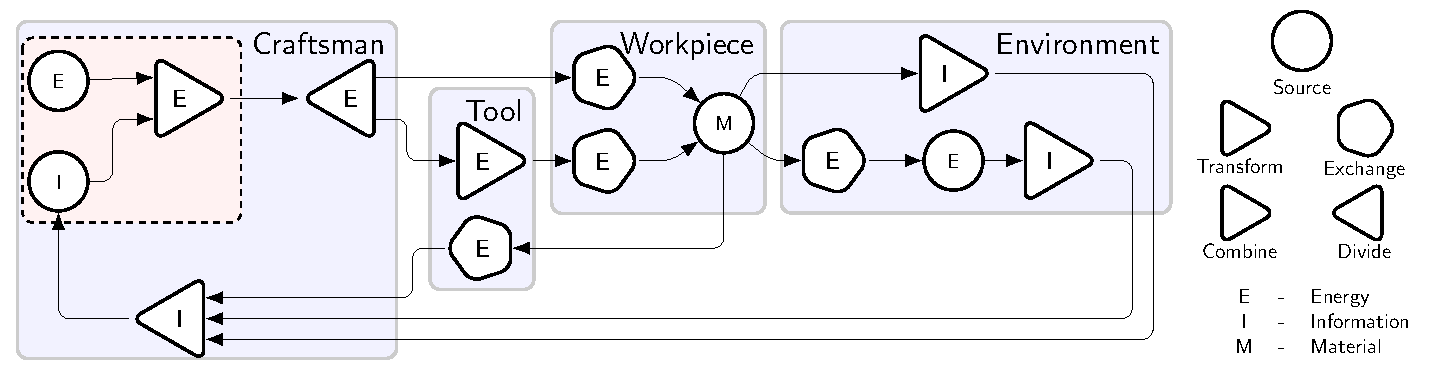
\includegraphics[width=\linewidth]{Images/DesignActivityPattern.pdf}  
  \caption{Design activity pattern}
  \label{fig:DAP}
\end{figure}

The coordinated movement of both the tool and workpiece are the primary elements of the decisive strategy that is consciously executed by a craftsman. As the craftsman works towards a target shape, this strategy will continually change and be adapted based on the sensory feedback received by the craftsman. Indeed, successful crafting is not just the application of movement and force to a workpiece, but requires qualities of care, judgement and dexterity \citep{Pye2008TheWorkmanship}, where dexterity is not just coordinated bodily movement, but considered as the craftman's response to the ever changing conditions of the workpiece \citep{Ingold2001BeyondSkill}. 

Understanding how this feedback information is processed to determine how manufacturing strategy is both specified and adapted is a widely covered topic and beyond the scope of this paper. Broadly, in information processing models such as Wickens \citep{Wickens2015EngineeringPerformance} and Endsley \citep{Endsley1995TowardSystems}, decisions are informed by perception of external stimuli, attention resources and both long term and working memory. These memories allow the craftsman to internalise a more detailed mental model of the process, allowing them to better match a set of decisions and actions that correspond to their desired outcome. However eliciting and contextualising this tacit knowledge that informs the decision making is challenging, as demonstrated by Wood in her analysis of craft knife makers \citep{wood2006transmitting}. %EGL: can you elaborate a bit on what this reference found? Why is it challenging? % DB: yes, I will revisit this. 



%Crafting, and its alignment with both art and design is a widely discussed topic \citep{risatti2009theory}. A useful focal point on craft is one by Roman author Vitruvius in \textit{De Architectura}, where the craftsmanship of the experienced architect is described in two elements, \textit{fabrica} and \textit{ratiocinatio} \citep{vitruvius_1999}.\textit{Ratiocinatio} is the underlying thinking and purpose of the object, rather than the concrete thing whereas \textit{Fabrica} is the craftsmanship that grows out of fabricating a material work when working toward a proposed design \citep{Poerschke2016}. It is held that the nature of craft lies in the perfect realization of a form before the work begins. We focus our attention on the \textit{fabrica} element of crafting; the process of creating a specified desired form from an initial workpiece and the inherent ability that enables the craftsman to carry this out successfully.



\newpage
\section{Mechanised Panel Beating} \label{sec:Mechanised}

Some of the versatile techniques established by the metalsmith have been used as the starting point for the development of new flexible processes. These new processes use traditional techniques and/or tooling to achieve a specified, desired geometry from blank sheets whilst eliminating the need for a human worker to physically operate the process and/or control the decision making elements.  Here, we review some of these new processes focusing on the hardware and control techniques used for production automation.

\subsection{Processes} \label{sec:MechanisedProcess}
\subsubsection*{Hammer}
Identifying processes that can be considered as automated hammering is not straightforward as the definition can be associated with a number of different incremental forming processes \citep{Emmens2010TheHistory}. Larger mechanised hammers are used in processing bulk material \citep{Lange1986HandbookForming} and kraftformers can be fitted with hammer tools for mechanised hammering (Section \ref{sec:Kraftformer}). Here, hammering is characterised by the sheet being loosely clamped around the edge and deformation occurring as a result of impact between a hammer and die, causing through thickness compressive stress, which in turn causes in-plane expansion, as specified in \citep{Allwood2006AJapan}. %[I THINK THIS DEFINITION IS TOO NARROW. SEE MY RESPONSE IN THE EMAIL. EGL]

There is only one example the author could find that fully meets these criteria for hammering. At the Loughborough intelligent automation centre, a process was developed using an industrial robot arm to manoeuvre a sheet through a kraftformer machine with a hammering tool fitted. A novel method to determine manufacturing strategy and to regulate the process is used - Mechatroforming \citep{Ilangovan2016AnForming}. Their technique specifies both the location and magnitude of the impact force on the workpiece required to shape the part. A database is used to specify this strategy, with data being gathered from tracking skilled craftsmen as well as finite element simulations. The exact structure of the database is not clear, but the system also uses sensors to scan the geometry of the sheet after a set number of impacts, enabling (near) real time feedback, alongside an impact force measurement sensor.

Though not directly replicating the craftsman's process, novel processes have been developed that take inspiration from manual hammering techniques. The technique of raising (figure \ref{fig:hammeringtechnique}) has inspired development of a novel mechanised spinning process which allows deeper bowls to be formed compared to traditional spinning \citep{Russo2020RaisingSpinning}. In this process, the deformation mechanism used during the manual technique is replicated, substituting the hammer and anvil with working and support rollers respectively. In another process developed by Yoon and Yang \citep{Yoon2001InvestigationMetal}, a hemispherical tool is used to punch sheets into a crevice, akin to hollowing. However this incremental punching process uses a different deformation mechanism than traditional hollowing and makes no reference to the traditional craftsman.

A number of processes utilise the aforementioned hammering techniques to deform material, though fail to meet our criteria as the sheet is clamped at the outer edge. These processes use a variety of manufacturing strategies, the most straightforward of which uses predetermined control to specify manufacturing strategy. Tanaka develops a process which clamps the outer boundary of the sheet and hammers a sheet, using a \textit{yani-dai} anvil - a plastic hammering support base with pine resin used in Japanese traditional artistic forging work \citep{Tanaka2005DevelopmentWorking}. Impact locations on the face of the sheet (toolpath strategy) are initially specified by mapping out the desired part shape using different mapping strategies (Spiralling inward/outward or contouring). The strategy is later developed to account for the developing deformed surface by using a parametric curve interpolation \citep{Asakawa2010DevelopmentProcess} and also to adjust the impact angle on the face of the sheet \citep{Takasugi2012DevelopmentShape}. A similar process is developed by Mori who uses a genetic algorithm to determine manufacturing strategy. The algorithm works by optimising manufacturing strategy for a desired geometry using an empirical model to simulate deformed geometry (specifically local curvature) for a given strategy. Data was obtained through FE simulation and physical experiments \citep{Mori1996DeterminationAlgorithm}. 

Some other processes that constrain the edge of the sheet use sensors as an integrated part of the manufacturing strategy.  For example, a two stage process developed by Mori by firstly hammering the part into a desired shape -  the strategy for which is selected from a database of strategies captured experimentally through a systematic variation of impact positions and depths, then secondly a camera is used to identify imperfections in the workpiece and the sheet reworked in these areas (akin to hollowing and planishing) \citep{Mori1998IncrementalDatabase}. The previously mentioned system developed by Tanaka is also developed to include online geometry feedback, resulting  in reduced deviations with desired part shape \citep{Tanaka2014DevelopmentHammering}. A machine is also developed at the Fraunhofer Institute where although manufacturing strategy is manually selected by the operator, a flexible holding system is used which adapts to the shape of part as it is formed \citep{Sharon2014FraunhoferReport}.

Processes described as variations of the well established incremental sheet forming (ISF) process are developed such that the sheet is repeatedly impacted (hammered) into position. These are sometimes referred to as incremental sheet punching (ISP) processes. Some example configurations of these processes include using a CNC or traditional mill to incrementally punch material with a static forming tool \citep{Wang2017IncrementalPath,Zhu2019ToolForming}, or use a bespoke reciprocating forming tool to hammer material, mounted either as an end effector to a 6 axis robot arm \citep{Schafer2005IncrementalRobots, Puzik2008IncrementalApplication, Luo2010AResults}, or to a CNC mill \citep{Asgari2017DesignDamper}. Manufacturing strategy is defined using analytically derived methods, such as the ones described in \citep{Sedighi2015AnProcess,Zhu2019ToolForming,Luo2010ASimulation}. However, these processes clamp the workpiece at the edge, do not use a supporting anvil, and make no reference to the traditional craftsman and their techniques.
 

\subsubsection*{Kraftformer} \label{sec:MechKraftformer}
Driving has received some limited attention by researchers, with a number of attempts to automate the manual process. In all known cases to the author, these are developed exclusively at the Technical University of Munich. All processes use a traditional Kraftformer with stretching tools installed, with the sheet manipulated using a 6 axis industrial robot arm. Acknowledging that this is the sole mechanical configuration, we focus at the different techniques used to define/control the manufacturing strategy, this being the trajectory of the arm and machine parameters.

Initially, the challenges associated with developing an automated solution using analytical methods were identified \citep{Golle2007DrivingProducts}. These were then replaced with `knowledge based' and `cognitive' approaches. Knowledge based systems derived new manufacturing strategies from strategies captured from physically formed %[SOMETHING MISSING HERE?]. 
`Cognitive' strategies used data collected from sensors to adapt the strategy when forming online in real time - similar to the traditional smith. An early example of this cognitive approach is the development of a system to simply assist manual driving. This allowed the worker to check the geometry of the part they are forming in real time with a desired geometry without having to remove the workpiece from the machine using cameras to scan in the geometry \citep{Scherer2010DrivingProducts}.

There are many ways in which the knowledge-based approach can be implemented. Initially, Hoffmann et al captured the manufacturing strategy used to manually form a sheet (impact forces and positions on the sheet). They then translated this data to allow for a industrial robot to handle the sheet and repeat the process, thus replicating the part  \citep{Hoffman2009AnHandling}. % An See [10] in `Automated driving by standardizing and scaling the manufacturing strategy'
Later, efforts were made to eliminate the need to explicitly capture a manufacturing strategy required to create a desired geometry. Initially, this was done by capturing and scaling the manufacturing strategy (the impact locations on the sheet) of a physically formed shape with a desired geometry \citep{Opritescu2012AutomatedStrategy}. % Automated driving by standardizing and scaling the manufacturing strategy
Subsequently, more sophisticated methods of scaling manufacturing strategy were used, utilising statistical methods \citep{Opritescu2016VariationVariance}  and Voronoi partitioning to subdivide toolpaths \citep{Hartmann2019Knowledge-basedPartitioning}. % Knowledge-based incremental sheet metal free-forming using probabilistic density functions and voronoi partitioning

Other analytical methods have been used to specify manufacturing processes. A novel, more computationally efficient approach using a purely geometric model to demonstrate the change of 3D-forms has been developed, where the respective forming parameters are identified through experiments \citep{Yang2011GeometricalProcess}. Model Predictive Control (MPC) has been used to define an optimal manufacturing strategy for shaping L shaped channel sections, based on an analytically derived deformation model \citep{Yang2009AutomatisierungProgramming}. The process has also been modelled using the finite element method \citep{Hoffmann2005StudiesMetal} but due to high computing time and the lack of flexibility in the modelling process, this method is not practicable for developing manufacturing strategies \citep{Scherer2013MethodenBlechumformung}. % SEE HERE IT'S A DIFFERENT TENSE AGAIN. MAKES FOR CHALLENGING READING

Recently, neural networks have been used to specify manufacturing strategy. Initially, shapes with limited curvature is along an L shaped profile are formed to reduce complexity \citep{Opritescu2015AutomatedApproach}. The network architecture was designed to input the desired geometry - specifically the curvature along the surface along with material parameters and the resulting output specifies manufacturing strategy (sheet trajectory through the tools). The network was trained using manufacturing strategies and geometries collected through experiments. This strategy was later developed towards more complex sheet geometries \citep{Hartmann2019AnFree-forming}.

\subsubsection*{English Wheel}
The English wheel has has received little attention, with only two known attempts to automate the process identified by the author. Both these mechanised variants use a traditional tool with the worker replaced by a 6 axis industrial robot arm. US company Zahner studied the feasibility of the process for industrial applications. Manufacturing strategy was defined using a rule based system, calculated by identifying patches of high Gaussian curvature on the surface of a desired form. A toolpath strategy was developed so that patches with greater curvature were wheeled more. Though no results were only published informally, doubly curved panels with curvature were produced and were ``in good alignment with predictions'' \citep{Vazquez2017RoboticWheeling,Vazquez2017EfficientSurfaces}. %[Could we mention here that we spoke to experts and they said they were wheeling incorrectly? YES, SAY THE STRATEGY APPEARING TO RELY ON BENDING (?) MORE THAN THINNING]

Having identified the complex nature of the wheeling process, Rossi and Nicholas used a neural network to generate a toolpath, citing the system's ability to capture complex behaviour that rule based systems cannot capture \citep{Rossi2018ModellingWheel, Rossi2018Re/LearningSurfaces}. The network was trained by tracking the formed geometry and the manufacturing strategy used to wheel four physically wheeled, digitised and augmented sheets. % EGL: NOT SURE WHAT AUGMENTED MEANS HERE
In carrying out the desired manufacturing strategy, a closed loop system was used (using a Kinect device) % WHAT IS THE ROLE OF THE KINECT HERE? SCANS THE PART? CLARIFY
to continuously adjust the position of the robot arm to account for the developing curvature of the sheet. The system architecture was constructed such that every new sheet that is fabricated is used to improve the neural network.

\subsubsection*{Spinning}

The process of hand spinning, as described in Section \ref{sec:Manual}, has known progressive mechanisation over the course of the second half of the 20$^{\text{th}}$ century. Two major requirements drove innovation: the need to spin larger and thicker parts, which required higher power than a human could deliver, and the need to spin larger quantities of parts faster \citep{Wong2003AProcesses}. This led, for example, to the use of the compound lever to exploit mechanical advantage and spin thicker workpieces; then, hydraulic lathes were introduced to apply even higher force. 

Speed and repeatability were improved by implementing template copying control and eventually computer numerical control (CNC) spinning machines in the 1970s. These innovations were the first steps towards automation: the human operator no longer had to manually direct the tool, but would program the tools to move using mechanical or electrical power. Curiously, however, Wong \textit{et al} \citet{Wong2003AProcesses} report that the need for experienced spinning operators with programming skills made CNC machines problematic. Thus, in the 1980s, teach-in/playback systems known as PNC (programmable numerical control) were introduced. In these systems, an experienced spinner makes the first part while their actions are recorded by a computer. Then, the tool trajectory is played back automatically to make the same parts. Thus, programming is not by means of numerical data, but by manual control. CNC spinning has remained advantageous only for parts that require a single tool pass to complete, such as cones. %[would be good to be able to include some references in this paragraph?]

In this case, the process is usually known as shear spinning, and leads to a reduction of the workpiece wall thickness while its diameter remains constant. The issue of automatically designing the trajectory of the tool (a key component in manufacturing strategy) to avoid failure of the workpiece has remained unsolved to this day. The extraordinary non-linearity of spinning precludes the possibility of any closed-form model \citep{Music2010ASpinning}. Therefore, researchers have attempted to optimise the design of the toolpath either by using statistical methods or by using numerical models. 

The former approach used case-based reasoning to select a suitable toolpath from an existing database based on the similarity between the new part to be spun and previous parts \citep{Henkenjohann2005AnProcess}. Then, it optimised the toolpath geometry using a technique called Adaptive Sequential Optimisation, which employs a statistical design of experiment methodology to reduce the number of trials needed to optimise the toolpath for the new part. This approach has two major limitations: it still requires many experiments to be performed for every new part, and it can only apply to parts with parameters that are within the range previously investigated. 

Numerical modelling was used by \citep{Polyblank2015ParametricSpinning} in a closed-loop strategy to correct the toolpath online to avoid failure of the workpiece by wrinkling or tearing. However, the long solution times of the finite element models made this system completely impractical. It would take over a year to design a full toolpath for a single part and a single material. 


 \citep{Wang2011ASpinning}??
 
 
\subsection{Mechanisation and Automation Technologies \label{sec:MechandAuto}}

A variety of processes are reviewed in section \ref{sec:MechanisedProcess}, each of which can be related back to a traditional technique used by the metal smith. On closer inspection, these new processes take inspiration from the traditional craftsman in one of three ways. Processes where physical and/or decision making elements are automated are defined as `Mechanised-Traditional' when a traditional technique and tooling are used to deform material or `Mechanised-Constrained' when traditional tooling or techniques is used, but is constrained in some manner - for example the sheet is constrained at the edges. Finally, `Variant' processes replicate similar deformation mechanics as the traditional processes, but the tooling/technique is substantially modified from its traditional form - for example ISP. 

In keeping with the theme of this review, we look more closely on mechanised processes. The mechanical hardware used to physically manipulate and actuate the sheet and/or tooling is predominantly carried out using industrial robot arms. [say why this is, and why it is good]. 

\renewcommand{\arraystretch}{1.2} 
\begin{table}[h] 
    \centering
    \resizebox{\linewidth}{!}{
        \rowcolors{1}{}{gray!10}
\begin{tabular}{lllcccccccc} \toprule
\rowcolor{white}
 &                                                                                                         & \multicolumn{1}{c}{}             & \multicolumn{3}{c}{Feedback Sensors}    & \multicolumn{5}{c}{Control data   context/source}                 \\
\cmidrule(lr){4-6}\cmidrule(lr){7-11}
\rowcolor{white}
               &                                                                                                 & Strategy Generation              & Visual         & Force      & Audio     & Heuristic & FE Simulation & Analytical & Experimental & Craftsman \\
\midrule
\multicolumn{11}{l}{\textbf{Hammer}} \\
			   & -                                                                                                               & Manual                           & \checkmark              & \checkmark          & \checkmark         & \checkmark         &               &            & \checkmark            & \checkmark         \\
               & \citep{Ilangovan2016AnForming}                                                                                  & Rule based (Mechatroforming)     & \checkmark              & \checkmark          &           & \checkmark         & \checkmark             &            & \checkmark            & \checkmark         \\
               & \citep{Tanaka2005DevelopmentWorking,Asakawa2010DevelopmentProcess,Takasugi2012DevelopmentShape}                 & \multicolumn{2}{l}{Rule-based (Tracing Part)}     &            &           & \checkmark         &               & \checkmark          & \checkmark            &           \\
               & \citep{Mori1996DeterminationAlgorithm}                                                                          & Genetic Algorithm                &                &            &           &           & \checkmark             &            & \checkmark            &           \\
               & \citep{Mori1998IncrementalDatabase}                                                                             & Database                         & \checkmark              &            &           &           &               & \checkmark          & \checkmark            &           \\
               & \citep{Wang2017IncrementalPath,Zhu2019ToolForming,Schafer2005IncrementalRobots,Puzik2008IncrementalApplication} & \multicolumn{2}{l}{Rule-Based (Novel Analytical)} &            &           &           &               &            & \checkmark            &           \\
               & \citep{Luo2010ASimulation}                                                                                      & \multicolumn{2}{l}{Rule-Based (Novel Analytical)} &            &           &           & \checkmark             &            & \checkmark            &           \\
               &                                                                                                         &                                  &                &            &           &           &               &            &              &           \\
\multicolumn{11}{l}{\textbf{Kraftformer}} \\
			   & -                                                                                                               & Manual                           & \checkmark              & \checkmark          & \checkmark         & \checkmark         &               &            & \checkmark            & \checkmark         \\
               & \citep{Scherer2010DrivingProducts}                                                                              & Manual                           & \checkmark              &            &           &           &               & \checkmark          &              &           \\
               & \citep{Hoffman2009AnHandling}                                                                                   & Predetermined                    &                &            &           &           &               &            & \checkmark            &           \\
               & \citep{Opritescu2012AutomatedStrategy,Opritescu2016VariationVariance,Hartmann2019Knowledge-basedPartitioning}   & \multicolumn{3}{l}{Rule-Based (Scaling Mfg strategy)}          &           &           &               & \checkmark          &              & \checkmark         \\
               & \citep{Yang2011GeometricalProcess}                                                                              & \multicolumn{2}{l}{Rule-Based (Novel Analytical)} &            &           &           &               & \checkmark          &              &           \\
               & \citep{Opritescu2015AutomatedApproach,Hartmann2019AnFree-forming}                                               & Neural Network                   &                &            &           &           &               &            & \checkmark            &           \\
               &                                                                                                         &                                  &                &            &           &           &               &            &              &           \\
\multicolumn{11}{l}{\textbf{English Wheel}} \\
			   & -                                                                                                               & Manual                           & \checkmark              & \checkmark          & \checkmark         & \checkmark         &               &            & \checkmark            & \checkmark         \\
               & \citep{Vazquez2017RoboticWheeling}                                                                              & \multicolumn{2}{l}{Rule Based (Novel Analytical)} &            &           & \checkmark         &               &            &              &           \\
               & \citep{Rossi2018ModellingWheel, Rossi2018Re/LearningSurfaces}                                                   & Neural Network                   & \checkmark              &            &           &           &               &            & \checkmark            &           \\
               &                                                                                                         &                                  &                &            &           &           &               &            &              &           \\
\multicolumn{11}{l}{\textbf{Spinning Lathe}} \\                                                                                                       &                                  &                &            &           &           &               &            &              &           & \\
               & -                                                                                                               & Manual                           & \checkmark              & \checkmark          & \checkmark         & \checkmark         &               &            & \checkmark            & \checkmark         \\
               & -                                                                                                               & Predetermined (CNC)              &                &            &           &           &               &            & \checkmark            &           \\
               & -                                                                                                               & Predetermined (PNC)              &                &            &           &           &               &            &              & \checkmark         \\
               & \citep{Henkenjohann2005AnProcess}                                                                               & Database                         &                &            &           &           &               &            & \checkmark            &           \\
               & \citep{Polyblank2015ParametricSpinning}                                                                         & Rule-Based (Novel..?)            &                &            &           &           & \checkmark             &            &              &    \\
\bottomrule			   
\end{tabular}
        }
    \caption{Automated process summary - Condensed }
    \label{tab:MechProcesses}
\end{table}

A summary of control characteristics for relevant `traditional' processes is given in Table \ref{tab:MechProcesses}. This outlines three main characteristics used to regulate the process. For comparison, manual techniques are also listed, using information collected in section \ref{sec:Manual}.
 

The control strategies used to regulate the process are categorised and listed. A predetermined control strategy indicates a strategy that is explicitly defined by an operator whereas a rule based strategy is one where the strategy is generated from a set of formula. Other control strategies are unambiguous in their definition. Sensors that feed back information to the system for real time processing are also shown for various data types. If no sensors are installed, then the process is considered open loop.

% [Comment on trends - Work carried out in section \ref{sec:tacitknowledge} demonstrated one of the key enabling characteristics of the craftsman is that they are very cognisant, making use of the different senses . This is reflected in the manual processes by the craftsman using many different senses to...]

The underlying knowledge/data that forms the basis of the control logic used in a process are also listed. These are arranged into five categories: Heuristic - when the underlying logic is based off a rational understanding of the process; Experimental - when knowledge is gained from a series of systematic physical experiments; Analytical - when knowledge is derived from a theoretical standpoint; FE - when data from simulation are used; Craftsman - when data captured from experienced craftsmen is used.

%Though all these processes strive toward full autonomy, none achieve this as worker input is still required at some level. Comparing processes autonomy is not straightforward as there are many different taxonomies available for ranking the level of autonomy (LoA) of a process \citep{Vagia2015AProposed, Frohm2008LevelsManufacturing}. Here,  Endsley's taxonomy is used \citep{Endsley1999LevelTask} as this specifically focuses on the automation of cognitive tasks (for example crafting) that require real time control \citep{Vagia2015AProposed}. The 10 LoA are shown in table \ref{tab:LoAEndsley}  and are determined by the allocation of four key roles being human (H) or computer (C) controlled.

%\begin{table}[h] 
  %  \centering
    %    \begin{tabular}{clcccc} \toprule
        &                               & \multicolumn{4}{c}{Roles}                                                            \\
\cmidrule(lr){3-6}
\multicolumn{2}{c}{Level of Automation} & \begin{tabular}[c]{@{}c@{}}Monitoring \\ System\end{tabular} & \begin{tabular}[c]{@{}c@{}}Generating \\ Strategy\end{tabular} & \begin{tabular}[c]{@{}c@{}}Selecting \\ Strategy\end{tabular} & \begin{tabular}[c]{@{}c@{}}Implementing \\ Strategy\end{tabular} \\
\cmidrule(lr){1-6}
1       & Manual Control                & H                 & H                   & H                  & H                     \\
2       & Action Support                & H/C               & H                   & H                  & H/C                   \\
3       & Batch Processing              & H/C               & H                   & H                  & C                     \\
4       & Shared Control                & H/C               & H/C                 & H                  & H/C                   \\
5       & Decision Support              & H/C               & H/C                 & H                  & C                     \\
6       & Blended Decision Making       & H/C               & H/C                 & H/C                & C                     \\
7       & Rigid System                  & H/C               & C                   & H                  & C                     \\
8       & Automated Decision Making     & H/C               & H/C                 & C                  & C                     \\
9       & Supervisory Control           & H/C               & C                   & C                  & C                     \\
10      & Full Automation               & C                 & C                   & C                  & C                    \\
\bottomrule
\end{tabular} 
    %\caption{Endsley's Level of Automation \citep{Endsley1999LevelTask}}
    %\label{tab:LoAEndsley}
%\end{table}





%Universal part production, akin to the skilled craftsman in their workshop has not yet been achieved, with most automated processes still requiring substantial human input on some level. Furthermore, with process combination not yet trialled, the individual deformation mechanics of each technique limit the levels of geometric variability achievable by each process. Here we review processes that are inspired by, or use traditional tooling/techniques to form parts and consider the hardware and control techniques used to automate production.

% Differences between experimental and craftsman
% Predetermined and rule based

%[I think it is worth discussing what we're trying to say in this section before we go any further and to also include any mechanised spinning processes. I think it is important to emphasise that most control systems now look to use closed loop control and database/ANN systems to account for the nonlinear behaviour observed in metalforming. This leads onto the next section, that these databases and NNs can be populated/trained through capturing data from skilled craftsmen. I think it would be good to also refer back to fig 22 in \citep{Allwood2016}]

%Nonetheless, a useful starting point is to list and contrast these processes. This allows for comparison of the underlying techniques, methods, sensors and mechanical characteristics for these processes. This allows us to both identify trends and identify useful technologies that might be cross compatible. Table \ref{tab:Process}, summarises applicable processes from section \ref{sec:MechanisedProcess} and summarises the different mechanical components and configurations that can be used to physically manipulate and actuate material as well as various different control strategies to regulate the process. For comparative purposes, the manual counterparts are also listed, using information collected in section \ref{sec:Manual}. 

%Assessing and comparing the merits of these different configurations would be challenging as there is no straightforward way to assess the autonomy of each mechanised variety. However using a previously mentioned classification by Frohm [ref], none of these processes are yet as versatile or efficient as their manual counterpart, so cannot be classified as fully autonomous. EGL: I wasn't sure what you were trying to say here. They are clearly not autonomous since they need human input. Also, what do you mean by merits here? Isn't the idea to look at the underlying techniques/methods/sensors/mechanical characteristics? Isn't that what the table is about? 


%The ultimate goal of autonomous flexible metal forming is 
%Though these processes strive toward a fully autonomous system, none of these achieve full autonomy as they still require worker input at some level. Assessing the merits of the different configurations used in attempting to achieve autonomy, there is no straightforward way of ranking which configurations/components are best.

% LoA - from Endsley
% Flexibility - 

% Flexibility
%		Low - Only a set number of shapes can be formed
%		Med - A small range of interpolated shapes can be formed (possibly in 1D/2D)
%		High - The full range of part shapes achievable by the manual counterpart process can be formed
% Degree of Approximation 

% Analogy with the skilled craftsman(?)
%		Novice - Repeating known actions to achieve known shapes
%		Apprentice - Has some understanding of the system and can define a strategy for forming a range of shapes
%		Expert - Has very good understanding of the system and can define a strategy for forming a greater range of shapes and also adapts this strategy instinctively if needed  



\newpage
\section{Learning from Craftsmen} \label{sec:Learning}

Though there are many automated adaptations of manual techniques used by the traditional smith, none of these processes are yet as versatile their manual counterpart. This implies that large amounts of knowledge, gained through years of experience are being discarded by not further observing the smith and how they operate these processes. Furthermore there are a number of overlooked techniques used by the smith that might serve as a useful starting point for novel process development. 

Understanding and capturing the skilled actions of the smith is challenging due to the tacit nature of the processes. However this presents an opportunity to develop new approaches to this challenge. In this section, we look at examples from both within and beyond the metal forming domain for technologies/methods of capturing and utilising the skilled actions of craftsmen, . There is a limited set of such activities in the literature, but they reveal the state of the art in this area and hint at future possibilities. 

\subsection{Learning from the community \label{sec:LfC}}
Despite a decline in professional craftsmen, the art of manual metal smithing is kept alive by an active community of artisans, circulating a wealth of knowledge through a range of widely accessible resources. Though useful to the hobbyist or apprentice, these resources are often overlooked by the academic community as the content lacks in technical understanding and explicitly defined process capabilities. Nevertheless, they can provide a useful starting point for describing techniques used to form shapes, advise on correct machine/tool configurations and give useful tips on how to avoid common mistakes the inexperienced workman or newly commissioned technology might face.

There are a number of written manuals aimed at training apprentice metal smith and hobbyists alike. Some of these manuals, such as Barr's sheet metal fabrication series \citep{Barr2013ProfessionalFabrication,Barr2019SheetProjects} detail step-by-step instructions for creating specific parts allowing other similar parts to be made by replicating procedures and slightly adjusting techniques. Other manuals, such as Timings \citep{Timings2008SheetMetalwork}, Thompson \citep{Thompson2007ManufacturingProfessionals} and Wakeford \citep{Wakeford1985SheetWork} take a more broad approach by detailing information about individual tools and techniques that can be used to create part shapes. Coppersmithing \citep{Fuller1904ArtForms} and silversmithing \citep{Hill2014ManufacturingProcesses} manuals provide details on similar techniques used to form material. There also exist manuals focusing specifically on the operation of a singular tool, such as the English wheel \citep{Longyard2014LearningWheel} and spinning lathe \citep{Tuells1912MetalUsed}, such is the complexity of opperating these tools.

Despite the thoroughness of these manuals, craftsmen often struggle to articulate the necessary tacit skills required for successful crafting \citep{Wood2009ACraftsmen}. This makes relaying information through manuscript challenging. Recorded instructional videos however give craftsmen the platform to more successfully convey the tacit nature of the task by enacting and thus demonstrating the process. Such resources are prevalent amongst a growing online community of craftsmen, allowing them to connect globally to share and record their expertise. Examples of such content are very common and for the interest of our readers, we can cite a few sources of such work such as Ron Corvell's Hand Metalworking series [See here http://covell.biz/dvds/hand-metalworking-dvds/]
and [...??]

Training courses where skilled craftsmen give interactive demonstrations and tutorials on tools and techniques are another excellent, underutilised resource. The authors note that the opportunity to observe a master craftsman at work and emulate their work under their supervision is an excellent route to adopting their good habits and developing an instinct for the relevant processes and materials. An experience instructor can also indicate the comparative difficulty of different techniques and part geometries. Very often, such comparisons are not obvious to a novice, or even to trained engineers without practical experience. Designers of automated processes have found it beneficial to familiarise themselves with the manual counterpart through attending such courses during the initial stages of process development \citep{Ilangovan2016AnForming}.

% EGL: YOU STARTED TALKING ABOUT DEMONSTRATION HERE AND ASKED FOR INPUT SO I ADDED A COUPLE OF SENTENCES. HOWEVER, THESE FIT BETTER IN THE NEXT SECTION, SO MOVE THERE AS YOU SEE FIT. THE POINT ABOUT LEARNING THE RELATIVE DIFFICULTY OF TECHNIQUES AND GEOMETRIES APPLIES TO DISCUSSIONS ON FORUMS ETC AS WELL THOUGH. OR TOPICS ON DIFFERENT TOOLS AND THEIR DIVERSE USES... 
%

\subsection{Learning from Demonstration} \label{sec:LfD} 
Much like the apprentice during the initial stages of their training, knowledge can be gained by observing a trained, skilled operator carrying out the process. Though section \ref{sec:LfC} briefly mentions how heuristic knowledge can be gained demonstration in in-person classes, here we focus on quantitative data that can be captured from skilled workers and used in the design or control of automated processes.

Systems acquiring new skills from human expert demonstrators using data acquired through sensors is not new, with Learning from Demonstration (LfD)  an already well established field \citep{Ravichandar2020RecentDemonstration}. 
However typical manufacturing applications within this field focus on more straightforward tasks such as robotic assembly \citep{Zhu2018RobotSurvey}. Despite this, we look for the various methods and technologies that can be used to capture the actions and techniques of the human operator can be used to capture the skilled actions of the craftsman.

Data can be collected using a vast range of cheap and readily available sensors, and there already exists an extensive review of sensors used to capture different metrics used in industrialised metalforming processes \citep{Allwood2016Closed-loopForming}. Here, we focus on capturing data specific to manual metal smithing processes, extending our search beyond the domain of metalforming. The design activity pattern in Figure \ref{fig:DAP} provides a useful starting point to identify the sorts of data that is critical to traditional forming and that should be captured. This include metrics that the craftsman controls: the trajectory of the tools and workpiece as well as machine configuration and also consider what the craftsman might be responding to: feedback from both the tool and workpiece in different manifestations - visual feedback, force feedback etc. 

\subsubsection{Capturing Geometry and Trajectories}
The trajectory and position of the sheet and tool are key elements of the manufacturing strategy. The topography of the sheet is also paramount, as during most metal smithing operations, this is often the defined target metric the craftsman is working toward. Capturing these visual metrics is therefor vital to understand the craftsman's manufacturing strategy.

Most processes reviewed in section \ref{sec:Mechanised} make use of some form of technology to capture the topology of the sheet. These are used either post process to analyse to the final form of the sheet, or in some cases used during the process as an integrated element of the control system. As demonstrated in the aforementioned review by Polybank \citep{Allwood2016Closed-loopForming} there are a vast array of sensors and methods that can be used to capture this type of data. For a given process the required sensing method will be selected based on factors such as resolution, processing time, availability and cost. 

There are fewer examples of technologies/methods used to capture the movement of the metal smith and their tools during manual processing. As part of the Mechatroforming approach, the trajectory of the sheet is tracked as it is manually worked  \citep{Ilangovan2016AnForming} using two vicon T-series cameras with the data collected used to populate the database control system. Similarly, the trajectory of a held hammer is tracked when striking the sheet to estimate the impact force on the sheet. The trajectory of the workpiece as it is manually worked is also captured as part of the cognitive driving strategies discussed in section \ref{sec:MechKraftformer}. 

Looking beyond the field of metalforming, there are a number of technologies and methods capable of tracking human motions, which can be used to subsequently capture tool/sheet trajectories to identify patterns/techniques. This is currently a rapidly expanding field, given recent interest in computer vision [ref?]. Data is collected through either worn sensors or through vision based systems.

Vision based systems collect data from sensors capturing colour (RGB) or a combination of colour and depth (RGBD) \citep{Zhang2019AMethods}. The challenge in using these types sensors lies in processing streams of data to identify movements and actions. Though off the shelf technologies are available with this capability built in (for example the Microsoft kinect), this can be achieved using generic, all-purpose cameras with data processed using one of the many different methods outlined in a number of comprehensive reviews \citep{Zhang2019AMethods,Beddiar2020Vision-basedSurvey}. Wearable technologies are electromechanical devices that attached to the body and record movements. Though the processing of data is more straightforward, these technologies are often more expensive and obtrusive than visual based systems. Nevertheless, there are again a number of comprehensive reviews into the state of the art of this type of technology used in medical \citep{Homayounfar2020WearableChallenges} and sport \citep{Taborri2020SportOverview} applications. [there are many more reviews we can add here]

\subsubsection{Capturing Forces (Haptics)}
In most manual forming processes, human operators are in physical contact with the sheet, whether directly with their limbs or indirectly through the tools they wield. In addition to visual information, then, they can also use haptic feedback to adjust and measure their actions. The word \textit{haptic} refers to anything to do with the sense of touch. During forming, this might be the evolving stiffness and strength of the workpiece, as well as intended or unintended vibrations or other mechanical effects can be monitored by craftsmen through this sense. Indeed, panel beaters often describe the sensation of feeling the material as it is worked. The response to haptic feedback can be either a conscious change in manufacturing strategy, or a more tacit change in the force applied to deform the workpiece. 

Haptic feedback is a prominent feature in manual spinning. During this process, the contact between the workpiece and the craftsman is mediated through the stick-shaped tool, which is held by the craftsman under the armpit and used in combination with a fulcrum pin to deform the rotating workpiece (see figure \ref{fig:SpinningProcess}). This haptic feedback can be used by the craftsman to gather important information on the workpiece, including thinning of the blank and hardening of the material. Crucially, force and vibration feedback are used to check that the workpiece is fixing itself tightly to the mandrel beneath, and to monitor its tendency to buckle. Though force feedback is used on many different automated spinning machines \citep{Arai2006Force-controlledMotors}, no study known to the authors has attempted to measure these forces during the manual process. However, \citep{Russo2019HapticSpinning} implemented a haptic spinning system to allow a human operator to control the working roller of a CNC spinning lathe, while providing them with force feedback from the workpiece. The system employs an off-the-shelf force-feedback joystick (known as Phantom Desktop and commercialised today by 3D Systems Inc.) in combination with loadcells installed on the two main motion axes of the roller. Using this system, the researchers have invited experience spinning craftsman and recorded their actions in a series of over 70 experimental trials, making the database available \citep{Russo2020ResearchSpinning}. The force data can be used as an alternative or together with the geometrical trajectory to design better toolpaths in spinning. Moreover, oscillations in the data can potentially be used to check whether wrinkling is about to happen. 

In an effort to begin to automate other manual manufacturing processes that are sensitive to haptic feedback, similar data has been collected . A mechatronic device developed by Kalt et al is used to measure force, torque, vibration on the tool during a manual polishing of metallic surfaces as well as tracking tool trajectory and feed rates \citep{Kalt2016TowardsOperation}. Similar tools are developed for use in capturing data for manual grinding \citep{Phan2018InstrumentationWorkpiece} and wood planing \citep{Montebelli2015OnTasks} [probably need to give some more detail on this?].


\subsubsection{Capturing Machine Configuration}
The craftsman regularly changes tools and adjust the machine configuration when crafting - for example changing forming tool during spinning or lower tool pressure when wheeling. Despite this, in most mechanised sheet forming applications, only one machine set up is considered, possibly to reduce complexity. However as different machine configurations are often manipulated by craftsman during the manual process, these must be considered as key elements in the manufacturing strategy.

Capturing the different machine configurations used during  manual smithing is trivial as these changes are often either indiscreet - such as tool changes, or measurable - such as changing lower anvil height when wheeling. However the author could find no examples of tracking these configurations during manual processing. Beyond metalforming however, Manorathna gives a prominent example of how manipulating machine parameters can be used to control the manufacturing process by tracking various parameters for expert and novice welders when working \citep{Manorathna2017HumanAutomation}. 

Though not explicitly learning from craftsman, systematic investigations into the effects of different machine configurations for some processes demonstrate the effect these can have on deformation. In spinning for example, the affect on tool forces and modes of failure has been investigated for different feed ratios (mandrel speed to tool feed rate) \citep{Sugar2016AnalysisSteels,Essa2010OptimizationAnalysis} and tool shapes \citep{El-Khabeery1991OnCups,Essa2010OptimizationAnalysis}. The effects of lower tool shape and height on both tool force and deformation characteristics during wheeling has also been investigated [Bowen et al ICTP 21 paper]. Furthermore, comprehensive reviews on the influence of process parameters on deformation in incremental sheet forming, a process often associated with the metalsmith processes \citep{Music2012TheTools}, suggest the importance of process configuration \citep{Gatea2016ReviewForming,Gohil2021ReviewProcess}.

\subsubsection{Learning from collected data}
Though data can be collected using a variety of cheap and readily available sensors, designers who are often not skilled craftsmen might not have the ability to interpret this data - that is to say, how are they to evaluate a good technique/set of data from a bad one, when they themselves are not experts? 
%Furthermore, additional challenges exist in collating data types to be used harmoniously. 
This challenge of eliciting techniques and knowledge from data acquired from skilled craftsmen is not limited to metal forming and there are different groups investigating how similar tacit knowledge can be understood and used.

A straightforward method of identifying skilled techniques is by analysing and comparing the actions of skilled and unskilled craftsmen carrying out identical tasks. Ikemoto studies the manufacturing strategies of 5 expert and 5 non-expert craftsmen repairing identically damaged car panel, using only a hammer.  Alongside completing the job to a higher standard, patterns emerge amongst experts for different metrics that are recorded, including strike positions \citep{Ikemoto2018ProcessRepair} and the time spent on tasks \citep{Ikemoto2016ARepair}. This begins to highlight the skilled actions of the expert craftsmen gained over years of experience that can be utilised in automated processes. Similar studies comparing skilled and novice workers have been undertaken for other manual manufacturing processes including machine configurations in a welding processes \citep{Manorathna2017HumanAutomation}, stroke directions in both hand lay-up of glass fibre reinforced composites \citep{Xie2016EffectMethod, Kikuchi2016ResearchLay-up} and biometric data (joint angles) during traditional stone knapping \citep{Rein2014MovementTraditions}. 

Having identified a skilled cohort, knowledge can be gained from identifying techniques and patterns that are repeated. An early example of this, is the identification of 15 commonly used gripping techniques used by skilled machinists to grasp objects \citep{Cutkosky1986ModellingHands} which nowadays is still widely used for the design of robot arm grippers \citep{Feix2016TheTypes}. This technique of analysing the actions of a skilled cohort has been used to identify 7 rules of spinning... [talk about Iaccopo's 7 rules of spinning]
Similar methods are used to identify techniques in manually layering pre-impregnated woven materials, using data collected from video analysis \citep{Elkington2015HandProcess, Elkington2015StudyingLayup} and later from quantitative movement tracking \citep{Prabhu2017DigitisationTechnology}. From this, new automated processes can be developed [EL, have you got the ref?]

There are a few notable cases where LfD has been used to control systems, where data has specifically been gathered from skilled craftsmen. Using force and positional data, toolpaths for automated production, using data collected from experts \citep{Ng2017CapturingGrinding}. [need to expand on this and can we find any more examples?]


% - - - - - - - - - - - - - - - - - - - - - - - - - - - - - - - - - - - - - - - - %
% Here I have included some other ref's which might fit in somewhere, but I am not sure where.
% \citep{Lamkull2009} - simulation of human movement. [still not sure how this one fits in exactly?]
% In \citep{Phan2020} a practical approach to estimate human joint stiffness during tooling tasks for the purpose of programming a robot by demonstration.


\section{Discussion}

By collectively reviewing an array of manual processes used by the craftsman in section \ref{sec:Manual}, a simple taxonomy of manual techniques used to form sheet metal parts is proposed - Figure \ref{fig:ManualTaxonomy}. These are grouped according to the tooling used, with each technique having a unique deformation mechanism and geometric forming capability. However the ad hoc nature of the manufacturing paradigm implies there are several more processes yet to be listed, which includes tools not considered in this review - bead rollers for example.

\begin{figure}[h]
	\centering
    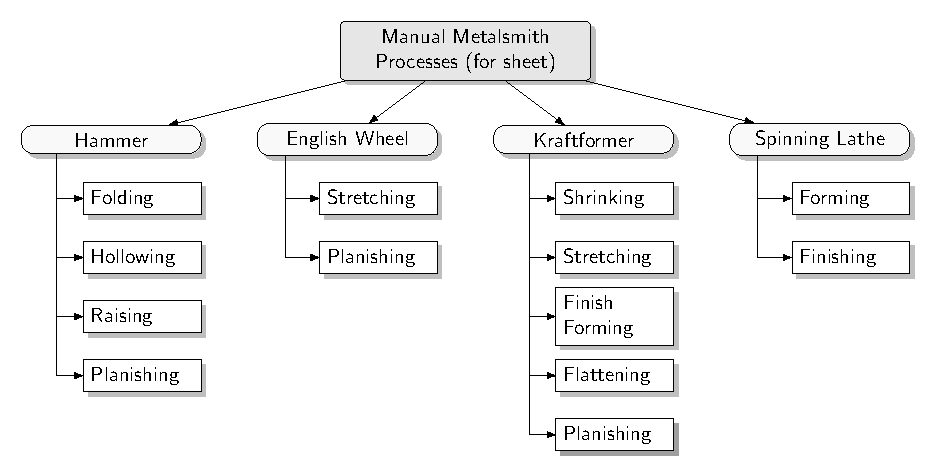
\includegraphics[]{Taxonomy.pdf}
    \caption{Taxonomy of manual processes [Could add * to processes that have been mechanised..? Also need to go back to section 1 and make sure each listed technique is mentioned]}
    \label{fig:ManualTaxonomy}
\end{figure}

Many of the techniques listed in the taxonomy remain ambiguous, with both deformation mechanism and specific procedure not yet explicitly defined. Interestingly however, it can be seen that many of these processes are essentially thinning/stretching or thickening/compressing the sheet locally to incrementally form shapes. A more thorough understanding of these traditional techniques developed over generations could lead to improved capabilities in modern processes as demonstrated by the fold-shearing and raising by spinning processes. 

Fundamental to the craftsman's versatility, is the ability to use a series of different processes to form a greater range of parts. Figure \ref{fig:ShapeDevBowl} shows anecdotally the various ways which the craftsman might form a deep bowl using different tools and techniques. [talk about the significance of this - why they might select certain tools (previous experience, other material properties, availability)]. Though individual processes have received attention, the effects of, and automation of process combination has yet to be attempted.

\begin{figure}[h]
    \centering
    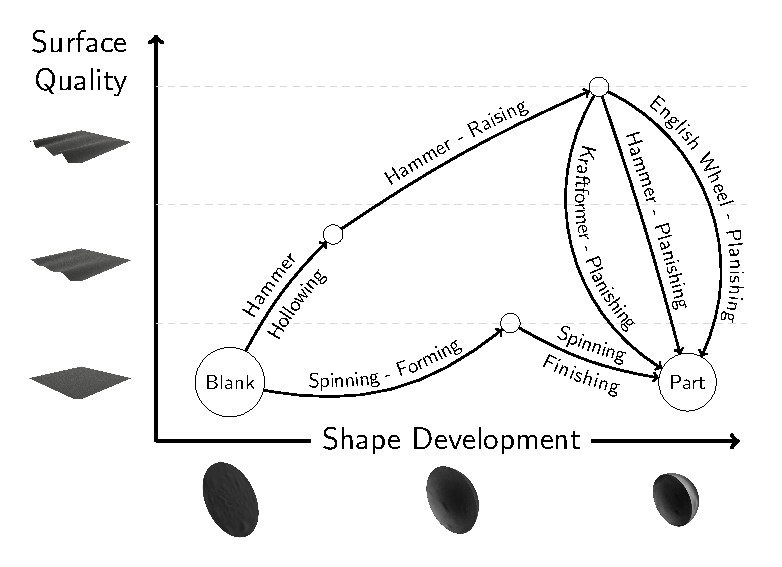
\includegraphics[width=0.6\textwidth]{Images/Bowl.pdf}
    \caption{Different manufacturing strategies using different techniques to form a deep bowl}
    \label{fig:ShapeDevBowl}
\end{figure}


\vspace{4em}
*From here to the end of the section needs finishing*
\vspace{4em}

merits of automating these manual processes is multifaceted. Alongside the inherent flexibility, with the sheet is not constrained at the boundary, springback and residual stresses (common challenges with many modern processes) is less of an issue. Automating processes is not a straightforward task

Without doubt, spinning has received the most attention from industry. [why]. Nevertheless, automated, reliable manufacturing strategy for universal part production is not yet achieved. 

A very limited subset of process parameters and sensing are usually included in these invented processes. Only a small subset of parameters are also trialled (forming force, tool shape etc)


 % EGL: I wonder if we should comments how all these processes are essentially thinning/stretching or thickening/compressing the sheet locally and we worry about the same failures in all of them (wrinkling, tearing). We can also say that because in all cases we have free boundaries, springback and residual stresses (common challenges with many modern processes) is less of an issue.
 
 %1 - There are many different traditional crafting processes.
%There is no taxonomy of processes
%The art of smithing is potentially being lost

%2 - In mechanised variant's the specific techniques are often overlooked - hammering is a prime example.
%Furthermore, there is no integration of processes to form an overall shape.
 
%3 -  Mechanised variant's are viable
%A very limited subset of process parameters and sensing are usually included in these invented processes. 
%Given the advances in technology, the process of physical mechanisation is straightforward. 


%\begin{enumerate}

%\item A lot of the panel beater's processes are ad hoc and/or not clearly defined. As well as scope for defining a more rigorous taxonomy, this also implies there are several opportunities to develop new techniques through closer observation of these craftsman.
%\item To achieve a system that is as versatile/flexible as the smith, a combination of processes will likely be needed. This will be challenging until individual processes have been fully established.
%\item With the decline in traditional smiths, the `art' of crafting (knowledge base of techniques and processes) is in danger of being lost. Establishing mechanised processes preserves these.
%\item There are technologies (sensors, control strategies) that have been used in some mechanised processes that could be applicable to other processes
%\item As mechanised processes are not yet as versatile as their manual counterpart, there is still a lot we can learn. This can be done using some of the many sensors used in the domain of LfD.
%\item The similarities between NNs and the craftsman, with regards the way they both learn through experience. 
%\item Database/ ANN approaches provide a method that can be populated by different data. For example, FE and human skill capture is used to inform the mechatroforming approach. These are useful as increasing computational powers should bring about more data rich simulations which could be used to populate databases in a cost effective manner.]
%\item The studies in \ref{tab:MechProcesses} support the earlier argument [what earlier arguement?] that a very limited subset of process parameters and sensing are usually included in these invented processes. Only a small subset of parameters are also trialled (forming force, tool shape etc)

%\end{enumerate}

\section{Conclusion}

For the first time, manual techniques used by the metal smith to form sheet metal parts have been considered collectively in an effort to begin to understand this traditional form of manufacturing. Using a range of academic and atypical resources, different techniques used by the smith to form sheet are collated, grouped by the respective tooling used to carry out the process. The review is limited to four tools - hammer, kraftformer, English wheel and spinning lathe. A taxonomy of individual processes is suggested, though many tools and techniques used by smith remain undocumented.

The flexibility of the smith is realised and a number of mechanised processes have been developed in pursuit of new, flexible forming processes. A review into these new processes is carried out, focusing on processes inspired by the four aforementioned tools....[to be finished]






%%References
\renewcommand{\bibname}{References}
%%Changes Bibliography to read References
\clearpage
%\bibliographystyle{agsm}
\bibliographystyle{unsrt}
%\bibliographystyle{ksfh_nat}
%%%% THIS IS WHERE YOU NEED TO EXPORT MENDLE TO %%%%
\bibliography{references}
%%%% THIS IS WHERE YOU NEED TO EXPORT MENDLE TO %%%%

%\end{multicols}
\end{document}